\documentclass[a4paper,12pt]{article}
\usepackage{epsfig,latexsym,amsmath,amssymb,epic,eepic,psfrag,subfigure,float,euscript,array}
\usepackage[latin1]{inputenc}
\usepackage{standalone}
\usepackage{tikz,pgf,pgfplots}

\newenvironment{exercise}[1][Uppgift]{\begin{trivlist} \item[\hskip
    \labelsep {\stepcounter{exerctr}\bfseries #1
      \arabic{exerctr}}]}{\end{trivlist}\vspace{10mm}}

\newcounter{exerctr}
\newcounter{abcctr}[exerctr]

\newcommand{\abc}{\noindent\vspace{1mm}\\ {\bf
    \stepcounter{abcctr}(\alph{abcctr})\ }}
\newcommand{\bbm}{\begin{bmatrix}}
\newcommand{\ebm}{\end{bmatrix}}
\newcommand{\point}[1]{\hfill {\bf (#1p)}\\ \vspace{-5mm}}
\newcommand{\ctrb}{\EuScript{S}}
\newcommand{\Lap}{\mathcal{L}}
\newcommand{\obsv}{\EuScript{O}}
\newcommand{\realdel}[1]{\text{Re}\left\{#1\right\}}
\newcommand{\imagdel}{\text{Im}}
\newcommand{\bC}{\mathbb{C}}
\newcommand{\bR}{\mathbb{R}}
\newcommand{\bmpv}{\begin{minipage}[t]}
\newcommand{\bmps}{\begin{minipage}[t]{45mm}}
\newcommand{\bmpm}{\begin{minipage}[t]{90mm}}
\newcommand{\bmpl}{\begin{minipage}[t]{140mm}}
\newcommand{\emp}{\end{minipage}}
\newcommand*{\zethree}{\big(z - \mexp{-3h}\big)}
\newcommand*{\mexp}[1]{\ensuremath{\mathrm{e}^{#1}}}

\addtolength{\topmargin}{-1cm}
\textheight 23.5cm
%\oddsidemargin 0.61cm
%\evensidemargin 0.61cm


\def\OctaveG{tf([0.5 1], [1 0 -1])}

\title{Computerized control partial exam 2 -- Dummy 1}
\author{Kjartan Halvorsen}

\begin{document}

\maketitle


\begin{description}
\item[Time] Whenever
\item[Place] Somewhere quiet
\item[Permitted aids] For the exam: The single colored page with your own notes, table of Laplace transforms, calculator
\end{description}

All answers should be readable and well motivated (if nothing else is written). Solutions/motivations should be written on the provided spaces in this exam. Use the last page if more space is needed.

\begin{center}
{\Large Good luck!} \\
\end{center}

\begin{tabular}{|l|l|}
\hline
\multicolumn{2}{|l|}{\bmpl
Matricula and name
\vspace*{14mm}
\emp}\\
\hline

\end{tabular}

\clearpage

%-----------------------------------------------------------------


\subsection*{Problem 1}
The plant in figure \ref{fig:2dof} is described by the pulse-transfer function
\begin{equation}
H(z) = \frac{0.8}{z(z-0.8)},
\end{equation}
which is a first order system followed by a time-delay of one sampling period.

Let the desired characteristic polynomial of the closed-loop system be
\begin{equation}
A_{cl}(z) = \underbrace{z(z-0.7)}_{A_c(z)}\underbrace{(z-0.5)}_{A_o(z)}
\end{equation}
and determine the polynomials \(R(z)\), \(S(z)\) and \(T(z)\) in an RST controller of the form in figure \ref{fig:2dof}. The pulse transfer function of the closed-loop system from the command signal \(u_c\) to \(y\) should be 
\begin{equation}
H_{c}(z) = \frac{0.3}{z(z-0.7)}.
\end{equation}
\begin{figure}
\begin{center}
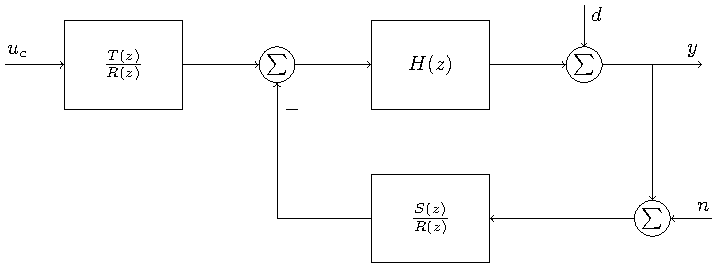
\includegraphics[width=0.7\linewidth]{../../homework/rst-block}
\caption{RST controller}
\label{fig:2dof}
\end{center}
\end{figure}

\noindent
\fbox{
\bmpl
{\bf Derivation:}\\
\vspace*{150mm}
\emp}



\clearpage
\subsection*{Problem 2}
(�\&W problem 5.2)
  The plant model is described by the pulse-transfer function
  \begin{equation}
  H(z) = \frac{1}{z+a}.
  \end{equation}
  Let the desired closed-loop system from the command input $u_c$ to $y$ be
  \begin{equation}
  H_m(z) = \frac{1+\alpha}{z+\alpha}
  \end{equation}
  and determine an RST controller of the structure given in figure \ref{fig:2dof}.

\noindent
\fbox{
\bmpl
{\bf Derivation:}\\
\vspace*{150mm}
\emp}

\newpage

\subsection*{Problem 3 - SKIP THIS }
The figure below shows the Nyquist curve for the dynamics of the pitch-direction of an aircraft. \textbf{Complete the skecth of the Bode plot for the same system.} The scale on the $ \omega $-axis is not
  important, as long as the amplitude and phase curve are
  in agreement.
\begin{center}
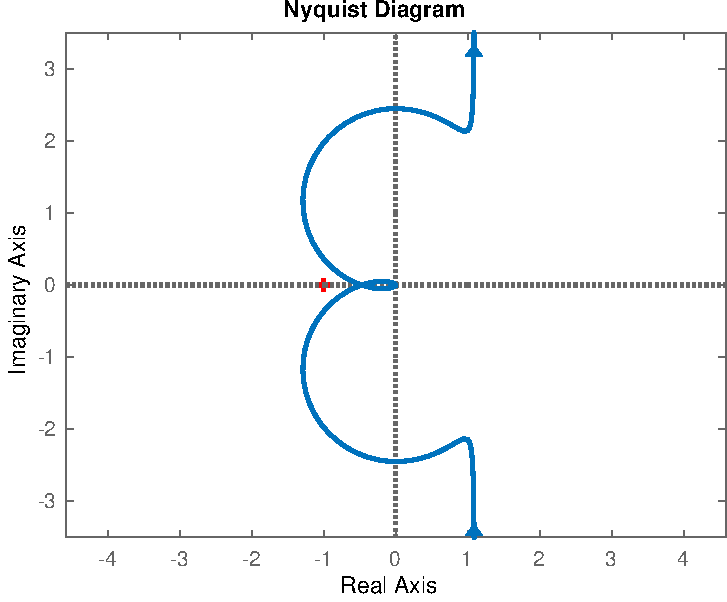
\includegraphics[width=0.6\linewidth]{nyq_bode_ex_nyq-crop}
\end{center}

\begin{center}
\fbox{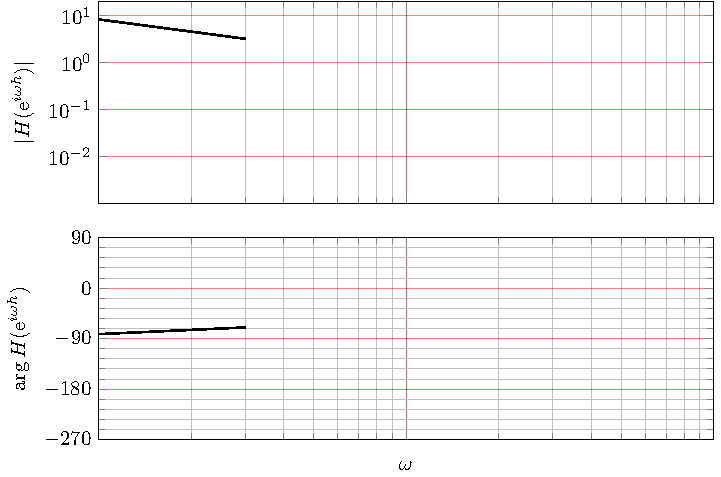
\includegraphics[width=0.999\linewidth]{nyq-bode-exercise}}
\end{center}

\clearpage

\subsection*{Problem 4}
The aircraft model from Problem 3 is controlled with a discrete-time lead compensator \(F(z) = K\frac{z-0.82}{z-0.25}\). 
\subsubsection*{(a)}
The figure below shows the root locus with respect to the gain $K$.
\textbf{Describe briefly the properties of the closed-loop system for different values of \(K\). Also: Mark, on the root locus in the figure, suitable closed-loop poles for the system (poles that can be obtained by some value of \(K\)).} 
\begin{center}
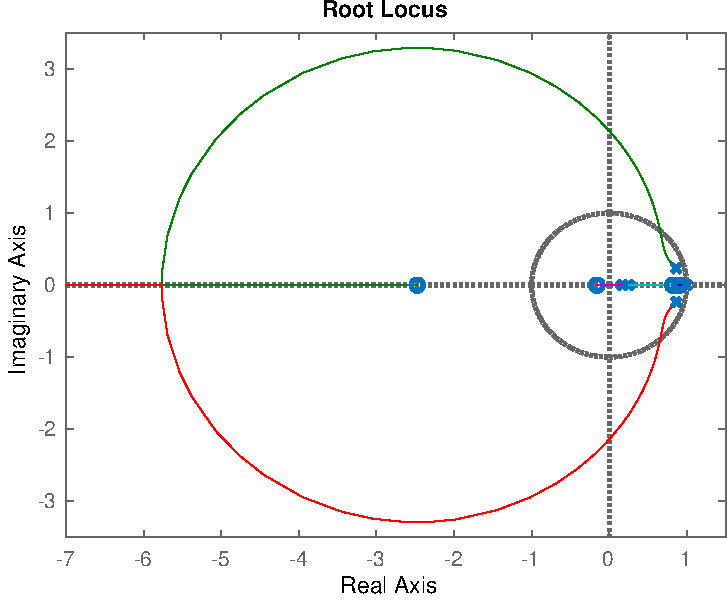
\includegraphics[width=0.49\linewidth]{discrete_aircraft_rlocus-crop}
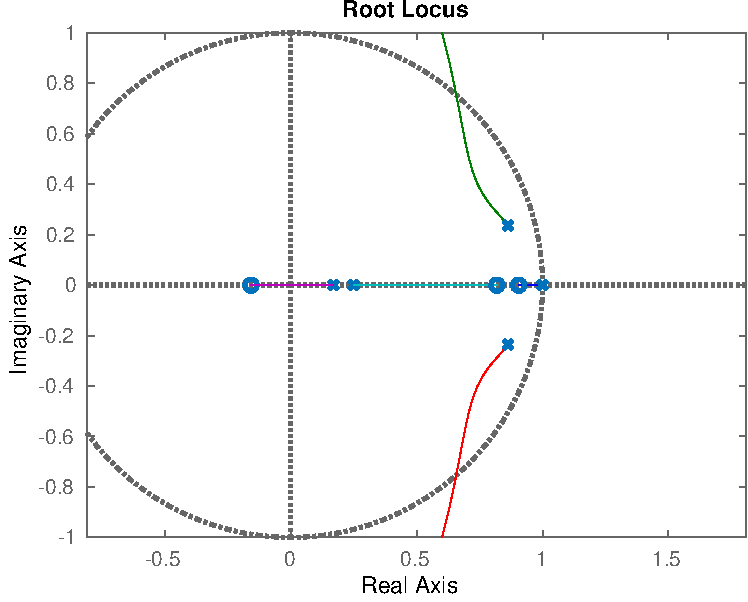
\includegraphics[width=0.49\linewidth]{discrete_aircraft_rlocus_zoom-crop}
\end{center}

\noindent
\fbox{
\bmpl
{\bf Description:}\\
\vspace*{80mm}
\emp}

\subsubsection*{(b)}
The figure below shows the Nyquist plot of the loop gain \(H_o(z) = F(z)H(z)\). \textbf{What is the phase margin and the amplitude margin? Mark in the figure and answer below.} 
\begin{center}
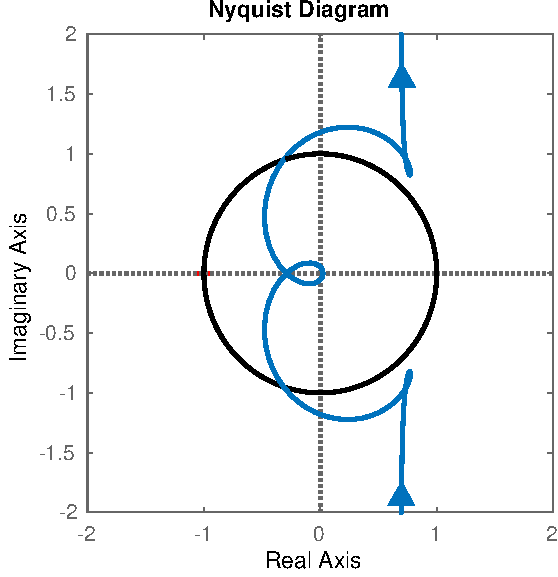
\includegraphics[width=0.6\linewidth]{discrete_aircraft_nyq-crop}
\end{center}

\noindent
\fbox{
\bmpl
{\bf $A_m$:}\\[3mm]
{\bf $\varphi_m$:}\\
\emp}





\clearpage

\noindent
{\bf If necessary,} you can continue your solutions on this page. Mark clearly which problem the solution corresponds to.


%\end{document}
%*****************************************************************
%*****************************************************************
\newpage
\setcounter{page}{1}

\section*{Solutions}
\subsection*{Problem 1}
The Diophantine equation
\[ A(z)R(z) + B(z)S(z) = A_c(z)A_o(z) \]
becomes
\[ \underbrace{z(z-0.8)}_{\text{order } 2}R(z) + \underbrace{0.8}_{\text{order } 0} S(z) = \underbrace{z^3-1.2z^2+0.35z }_{\text{order } 3}, \]
It is clear that to obtain the desired characteristic polynomial on the right hand side of the equation, we must choose a first-order controller:
\begin{align*}
R(z) &= z + r_1\\
S(z) &= s_0z + s_1.
\end{align*}
This gives the Diophantine equation
\[ z^3 + (r1 - 0.8)z^2 - 0.8r1z + 0.8s_0z + 0.8s_1 = z^3-1.2z^2+0.35z, \]
which gives the three equations 
\begin{align*}
r_1 -0.8 &= -1.2\\
-0.8r_1 + 0.8s_0 &= 0.35\\
0.8s1 &= 0,
\end{align*}
with solution
\begin{align*}
r_1  &= -0.4\\
s_0 &= 0.0375\\
s_1 &= 0.
\end{align*}

The pulse transfer function from \(u_c\) to \(y\) is 
\begin{equation*}
 \begin{split}
 H_c(z) &= \frac{\frac{T}{R}\frac{B}{A}}{1 + \frac{B}{A}\frac{S}{R}}\\
        &= \frac{TB}{AR+BS} = \frac{TB}{A_cA_o}.
 \end{split}
\end{equation*}
The polynomial \(T(z)\) is chosen to cancel the observer pole, so we have
\[ T(z) = t_0 A_o(z)\]
and
\[ H_c(z) = \frac{t_0B(z)}{A_c{z}} = \frac{0.8t_0}{z(z-0.7)}. \]
The  latter expression should be equal to 
\[ \frac{0.3}{z(z-0.7)}, \]
So,
\[t_0 = 0.3/0.8 = 0.375. \]

In summary, the controller is given by the three polynomials
\begin{align*}
R(z) &= z+r_1 = z-0.4\\
S(z) &= s_0z + s_1 = 0.0375z\\
T(z) &= t_0A_o(z) = 0.375(z - 0.5).
\end{align*}
\subsection*{Problem 2}
We have 
\[
    H(z) = \frac{B(z)}{A(z)} = \frac{1}{z + a}.
 \]
Further, the desired polynomial \(A_c(z) = z+\alpha\) is given. So the RHS of the Diophantine equation becomes
\[ A_{cl}(z) = A_c(z)A_o(z) = (z+\alpha) A_o(z). \]
and the whole equation becomes
\[ (z+a) R(z) + S(z) = (z+\alpha) A_o(z). \]
We need to decide the order of the observer polynomial in order to determine the order of the controller polynomials and then solve the Diophantine equation. 

The simplest controller is obtained with the choice \(A_o(z)=1\). This gives the equation
\[ (z+a) R(z) + S(z) = (z+\alpha). \]
Since the right hand side has order one, the left hand side must also have order one. This gives that \(R(z)\) must be of order zero. Further, \(S(z)\) cannot be of higher order than \(R(z)\), so we must have the controller polynomials
\[ R(z) = r_0, \quad S(z) = s_0. \]
We get the equation
\[ (z+a)r_0 + s_0 = (z+\alpha), \]
which leads to the equations
\begin{align}
r_0 &= 1\\
a r_0 + s_0 &= \alpha,
\end{align}
with solution
\begin{align}
r_0 &= 1\\
s_0 = \alpha-a
\end{align}

We must also determine the \(T\) polynomial. The pulse transfer function from \(u_c\) to \(y\) is given by
\[ H_c(z) = \frac{T(z)B(z)}{A_c(z)A_o(z)}. \]
From the specification, this is to be equal to 
\[ H_m(z) = \frac{1+\alpha}{z+\alpha}. \]
We have \(A_o(z) = 1\) and \(B(z) = 1\), so we get the equation
\[ \frac{T(z)}{z+\alpha} = \frac{1+\alpha}{z+\alpha}, \]
and hence
\[ T(z) = 1 + \alpha. \]

The resulting controller becomes 
\begin{align}
 R(z) U &= T(z)U_c - S(z)Y\\
 U &= (1+\alpha)U_c - (\alpha-a)Y\\
\end{align}
or, written as a difference equation
\begin{align}
u(kh) &= (1+\alpha)u_c(kh) - (\alpha-a)y(kh).
\end{align}

\subsection*{Problem 3}
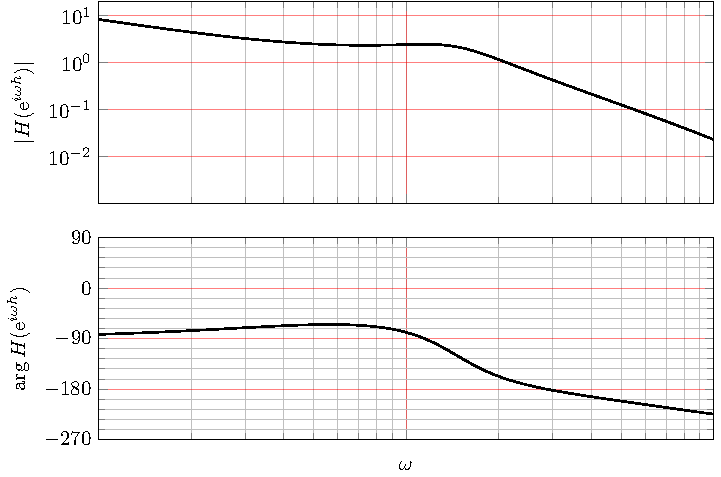
\includegraphics[width=0.9\linewidth]{nyq-bode-exercise-sol}

\subsection*{Problem 4}

\subsubsection*{(a)}
We have starting points in $1$, in $0.1$ (approximately) and two complex-conjugated starting points. For small values of $K$ the closed-loop poles are close to the starting points, and so the system has a slow dominating pole close to $1$. This pole remains rather close to $1$, since it goes towards the ending point in 0.85. As we increase $K$ the system will stay stable for a while. It will be oscillatory due to the complex conjugated poles (these have a damping of 0.4, approximately), and the response will be dominated by the slow real pole. There is also a fast pole much closer to the origin, but this will not affect the behaviour much.  For larger values of $K$, the two complex-conjugated poles break out of the unit circle and the closed-loop system becomes unstable. 

Suitable closed-loop poles

\begin{tikzpicture}
    \node[anchor=south west,inner sep=0] at (0,0) {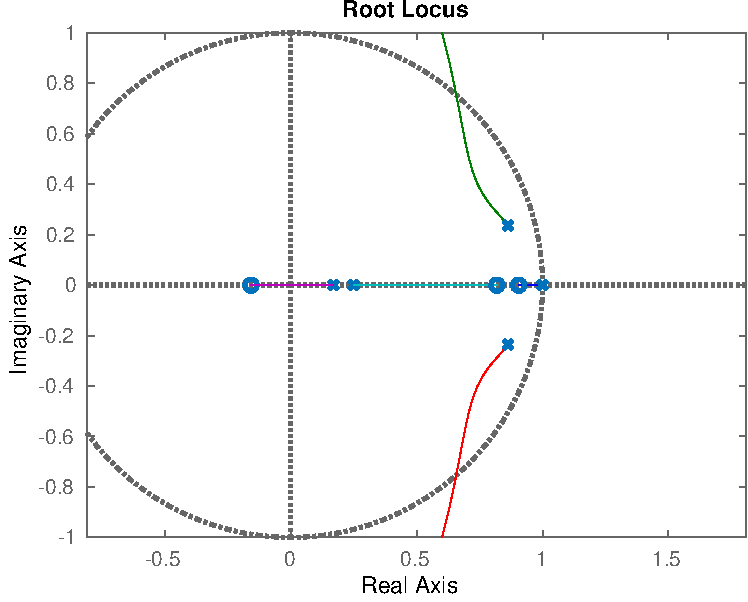
\includegraphics[width=0.79\linewidth]{discrete_aircraft_rlocus_zoom-crop}};
\node[black] at (6.89,3.1) {\huge $\times$};
\node[black] at (6.89,6.1) {\huge $\times$};
\node[black] at (4.6,4.6) {\huge $\times$};
\node[black] at (7.7,4.6) {\huge $\times$};
\end{tikzpicture} 

\subsubsection*{(b)}

\begin{tikzpicture}
    \node[anchor=south west,inner sep=0] at (0,0) {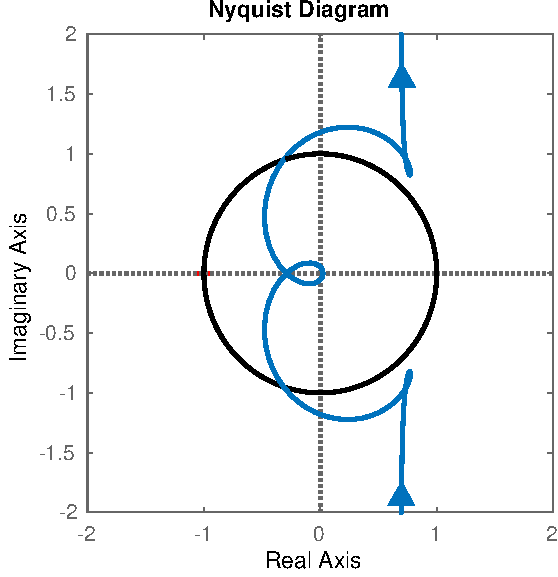
\includegraphics[width=0.7\linewidth]{discrete_aircraft_nyq-crop}};
\node[coordinate, pin={[pin distance=2cm]135:{$\frac{1}{A_m} \approx 0.35$}}] at (4.89,5.2) {};
\node[coordinate, pin={[pin distance=1cm]-135:{$\varphi_m \approx 70^\circ$}}] at (4.8,3.3) {};
\end{tikzpicture} 


\end{document} 
